% !TEX root = ../Bachelorthesis.tex
%
%************************************************
% Einführung
%************************************************
\chapter{Einführung}
\label{sec:Einfuehrung}

Springer Nature ist ein weltweit führender Verlag für Forschungs-, Bildungs- und Fachliteratur mit einer breiten Palette an angesehenen und bekannten Marken und zudem der größte Verlag für Wissenschaftsbücher. Für Springer Nature ist es darum wichtig, auf ihren Web-Applikationen eine Suche anbieten zu können, die Suchintentionen erkennt und möglichst schnell zum gesuchten Content leitet. Die Suche wird vor allem als Hilfsmittel zur Navigation und Suche nach Literatur und Dienstleistungen genutzt. Durch die vielen von Springer Nature publizierten Zeitschriften und Querverweise in Artikeln, wird sie aber auch oft zur Suche nach Issues\footnote{Nummer der Zeitschriftenausgabe, in der sich der Artikel befindet.} und Artikeln verwendet sowie als Hilfestellung um Diagnosen zu Krankheitsbilder stellen zu können.
\\
\\
Springer Nature sammelt viele User-Tracking-Daten und dadurch viel Wissen über das Verhalten der User auf ihrer Suche, lässt dieses Wissen jedoch nicht in ihre Suche einfließen. In dieser Arbeit wollen wir untersuchen, ob mithilfe dieses Wissens, die Suche optimiert werden kann.

\section{Aufbau der Suche bei Springer Nature}
\label{sec:Einfuehrung:AufbauSucheBeiSpringerNature}

\subsubsection{White Label Applikation mit Solr-Suche}
\label{sec:Einfuehrung:AufbauSucheBeiSpringerNature:WhiteLabelApplikationSolr-Suche}

Damit die verschiedenen Verlage und Zeitschriften der Verlagsgruppe Springer Nature ihre Produkte und Dienstleistungen online anbieten können nutzt Springer Nature eine inhouse entwickelte White Label Applikation\footnote{Eine White Label Applikation ist eine wiederverwendbare und agil erweiterbare Applikation}. Die White Label Applikation verwendet \textit{Apache Solr}\footnote{http://lucene.apache.org/solr} als Suchplattform. Die Solr dient hierbei als eine der Schnittstellen zwischen dem Content-Pool von Springer Nature und der Core-Applikation. Bei dem vom Content-Pool gelieferten Content, handelt es sich um vom Springer Nature-Verlag publizierte Zeitschriften, Artikel, Bücher, Chapters und redaktionelle Inhalte.

\subsubsection{User-Tracking mit Webtrekk}
\label{sec:Einfuehrung:AufbauSucheBeiSpringerNature:Webtrekk}

Um das Verhalten der User auf ihren Web-Applikationen zu tracken verwendet Springer Nature das Analysetool Webtrekk\footnote{https://www.webtrekk.com}. Die daraus resultierenden Reports bieten unter anderem die Möglichkeit, \textit{Suchquery-Logs} und \textit{Click-Trough-Rates} (CTR)\footnote{Kennzahl um die Anzahl der Klicks auf Links im Verhältnis zu den gesamten Impressionen darzustellen} der User auszuwerten.

\pagebreak

\subsubsection{Architektur}
\label{sec:Einfuehrung:AufbauSucheBeiSpringerNature:Architektur}

In Abb. \ref{fig:SucheSpringerNature} ist die Suche nochmals grafisch aufbereitet:

\begin{figure}[H]
\centering
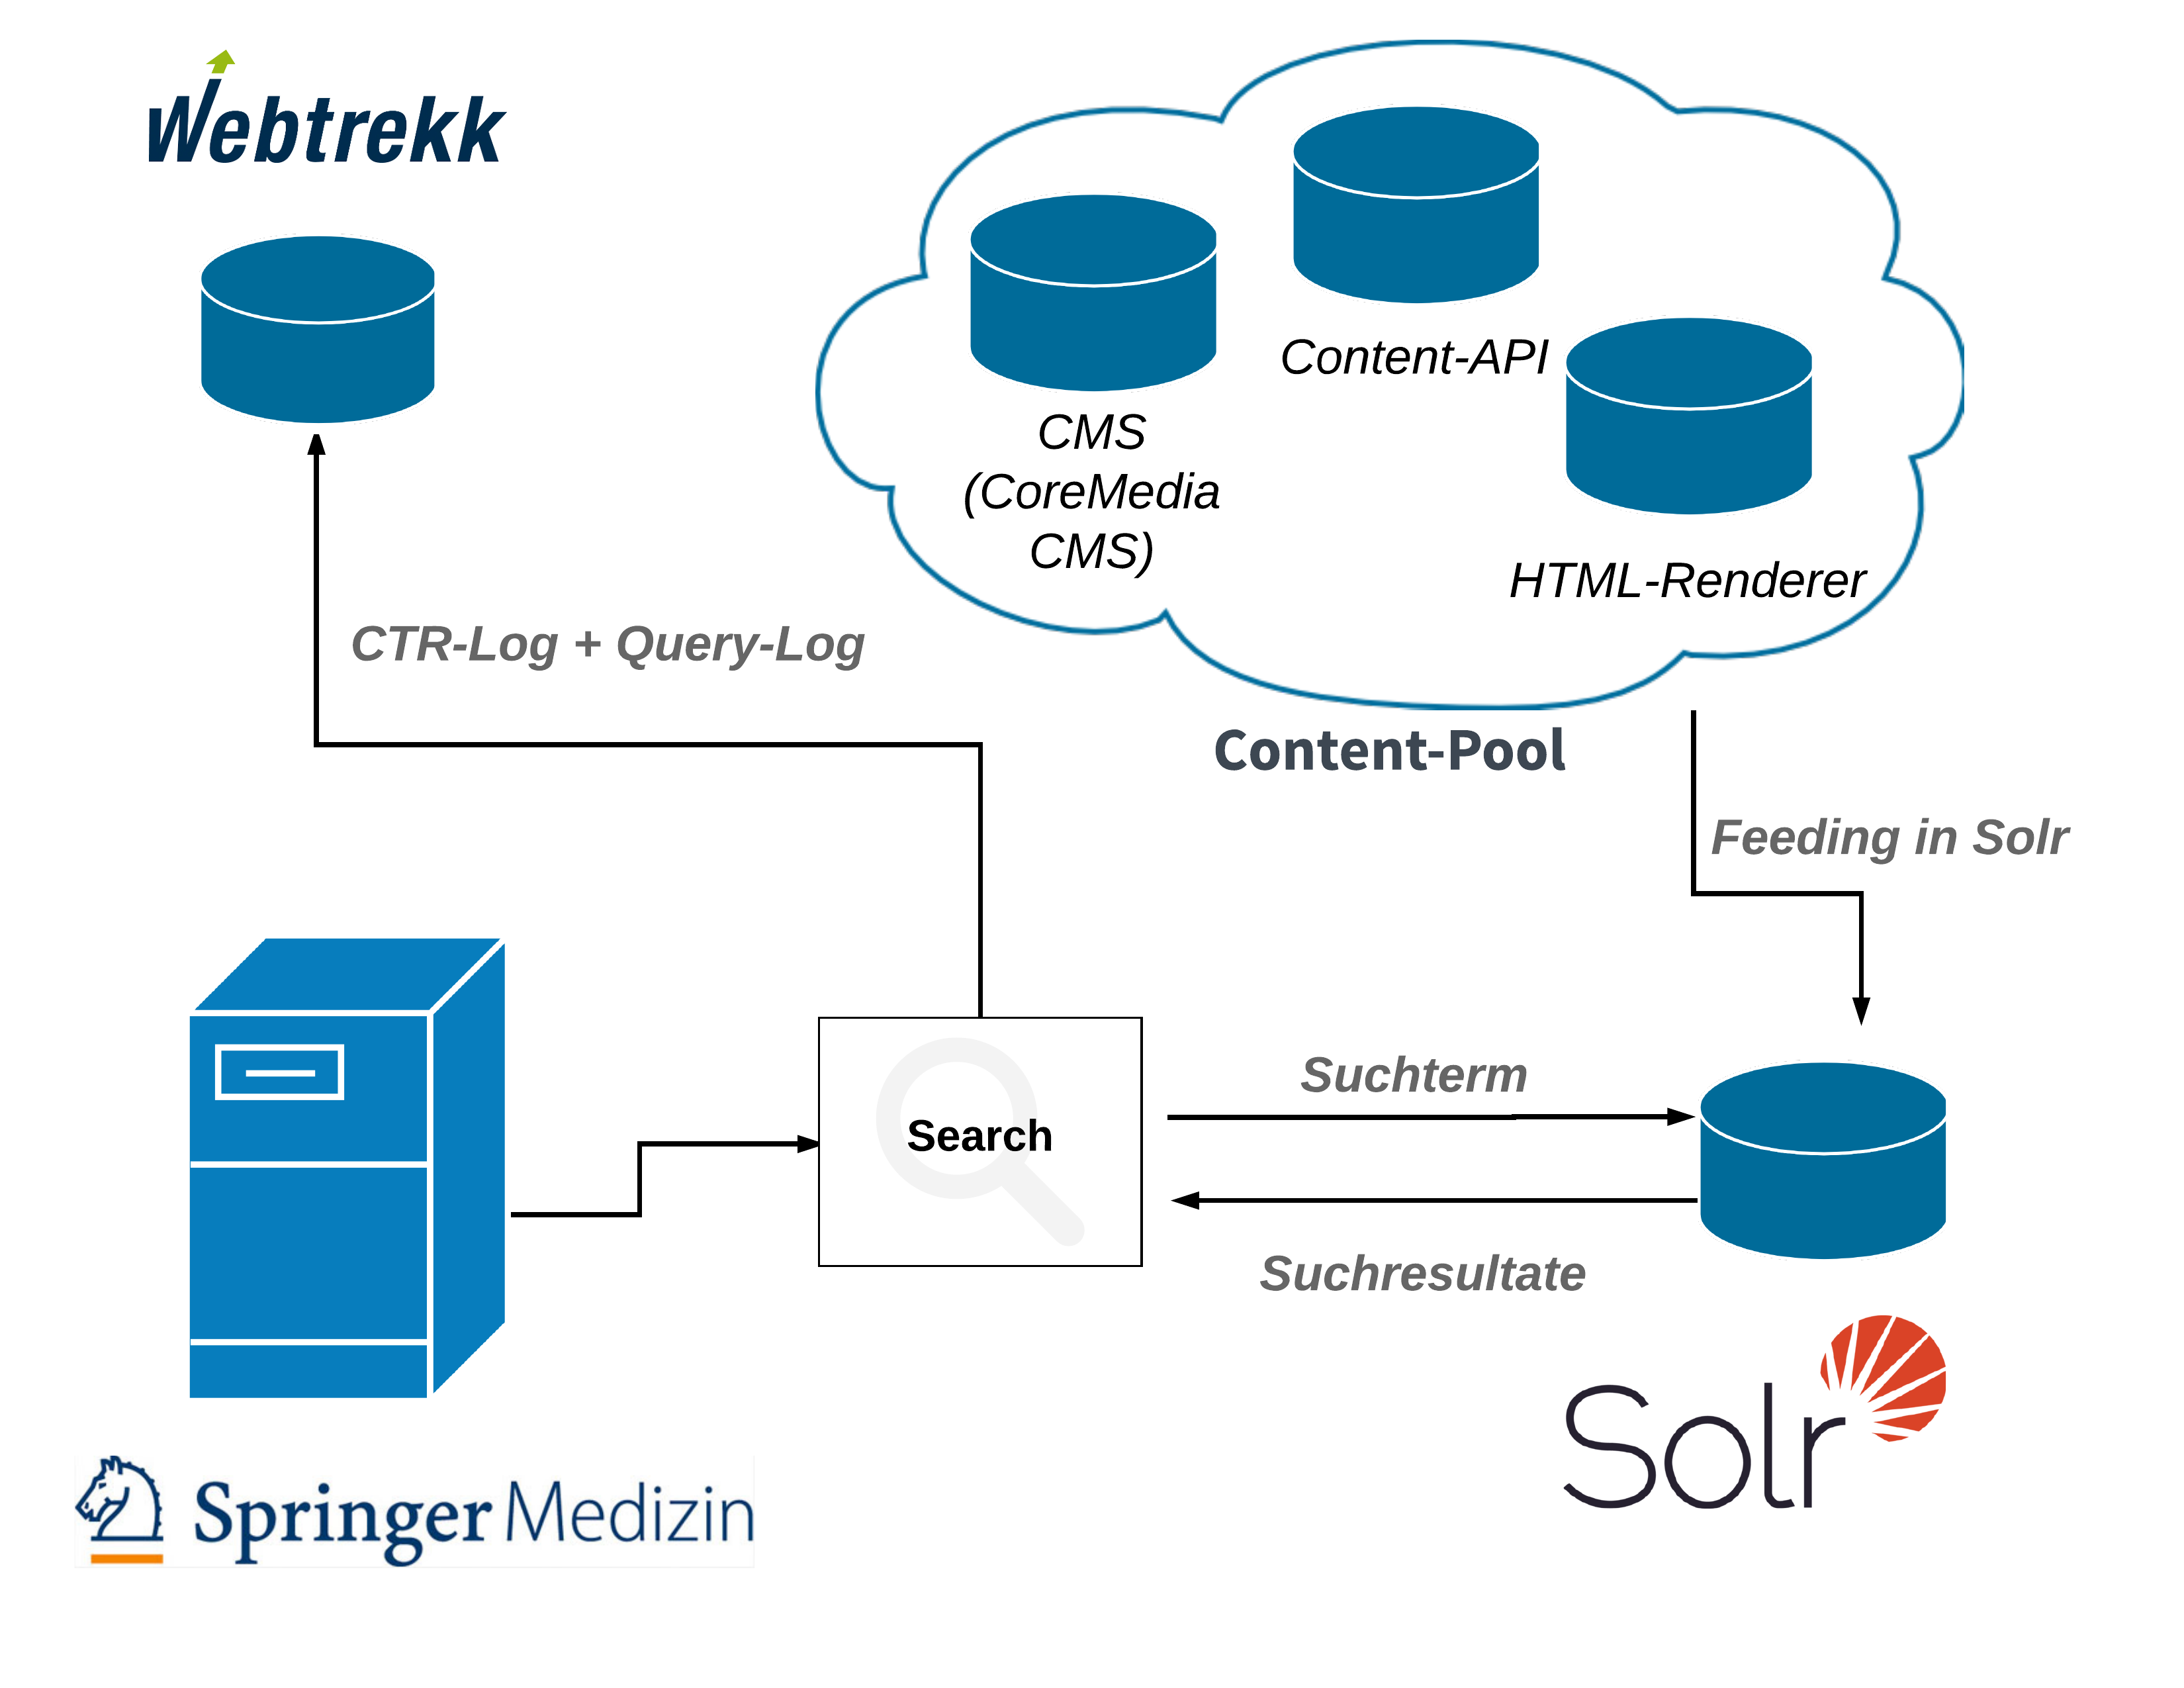
\includegraphics[width=0.5\linewidth]{gfx/AufbauSucheSpringerNature}
\caption[Aufbau der Suche bei Springer Nature]{Aufbau der Suche bei Springer Nature}
\label{fig:SucheSpringerNature}
\end{figure}

\section{Das große Problem}
\label{sec:Einfuehrung:Problemstellung}

\subsubsection{Keine Userrelevanz in der Suche}
\label{sec:Einfuehrung:Problemstellung:Userrelevanz}

Die User von Springermedizin suchen oft mit einschlägig, fundierten Fachbegriffen nach den neuesten und relevantesten Zeitschriften, Bücher oder Publikationen. Die zeitlich aktuellsten Suchtreffer zu finden ist für Springermedizin kein Problem. Die für den User \textit{relevantesten} jedoch schon.

\subsubsection{Der Springer Nature Stakeholder: Springermedizin setzt auf Webtrekk}
\label{sec:Einfuehrung:Problemstellung:Springermedizin}

Zu den Stakeholder\footnote{Bezeichnet Springer Nature interne Kunden, die ein Interesse am Ergebnis der White Label Applikation haben} der in Kapitel \ref{sec:Einfuehrung:AufbauSucheBeiSpringerNature:WhiteLabelApplikationSolr-Suche} angesprochenen White Label Applikation gehört \textit{Springermedizin}\footnote{https://www.springermedizin.de/}. Springermedizin ist ein Fortbildungs- und Informationsportal für Ärzte. Mithilfe von Webanalysten und Webtrekk versucht Springermedizin das Marketing ihres Webauftrittes zu verbessern und ist sehr interessiert an neuen Ansätzen, um die gesammelten Tracking-Daten besser einzusetzen. In dieser Arbeit wird darum der Fokus auf die Suche von Springermedizin gesetzt. 
 

\subsubsection{Der fast gläserne User}
\label{sec:Einfuehrung:Problemstellung:Glaeserne-User}

Springermedizin sammelt Tracking-Daten über jegliche Aktivitäten auf deren Applikationen und investiert Zeit und Geld in die Individualisierung der Analysedaten auf Webtrekk. Mittlerweile sind knapp 30 Custom-Parameter\footnote{Individuell erzeugte Parameter für Reports und Analysen} auf Webtrekk angelegt um genau die Daten zu tracken, die sie über das Verhalten der User auf ihrer Applikationen wissen wollen. Dadurch ensteht ein fast \glqq gläsernen User\grqq{}.

\section{Ziel der Arbeit}
\label{sec:Einfuehrung:ZielArbeit}

\subsection{Suchoptimierung durch Click-Trough-Daten}
\label{sec:Einfuehrung:ZielArbeit:Suchoptimierung}

In dieser Arbeit werden wird untersuchen, ob mithilfe der von Springermedizin gesammelten Click-Trough-Daten deren Suche verbessert werden kann. Im Idealfall entsprechend die gesammelten Click-Trough-Daten der Suchresultate, der Userrelevanz der einzelnen Dokumente\footnote{Als Dokumente werden die einzelnen Suchresultate bezeichnet}.

\subsubsection{Annahmen}
\label{sec:Einfuehrung:ZielArbeit:Suchoptimierung:Annahmen}

Wir gehen dabei von folgenden Annahmen aus. Relevante Dokumente sind wichtiger als nicht relevante Dokumente. Eine Suchergebnis ist dann gut, wenn die relevanten Ergebnisse vor den nicht relevanten Ergebnisse auftauchen. 

\subsection{Abbildung auf Springermedizin-Umfeld}
\label{sec:Einfuehrung:ZielArbeit:AbbildungSpringermedizinUmfeld}

\subsubsection{Potential von Userrelevanzen in der Suchoptimierung analysieren}
\label{sec:Einfuehrung:ZielArbeit:Potential}

Die Analyse von User-Tracking-Daten bietet viel Potential bezogen auf Userrelevanzen. Sind anhand des hier umgesetzten Lösungsansatz Verbesserungen in der Qualität der Suche zu verzeichnen, möchte Springer in Zukunft vermehrt User-Tracking-Daten in die Suche einfließen lassen. Diese Arbeit könnte dann als Fundament für weitere Lösungsansätze dienen.

\subsubsection{Bekanntes und wirkungsvolles Information Retrieval Verfahren}
\label{sec:Einfuehrung:ZielArbeit:AbbildungSpringermedizinUmfeld:InformationRetrievalVerfahren}

Suchoptimierung mittels Userrelevanz ist ein bekanntes und nicht ganz triviales, aber relativ wirkungsvolles, Information Retrieval Verfahren (siehe \cite{IWUSBI}). Seit Mitte der 2000er Jahre wird mithilfe dieses Verfahrens versucht, Suchmaschinen zu verbessern. Aus dieser Zeit stammen auch die ersten Ansätze um mithilfe von Click-Trough-Daten die Userrelevanz der Suchergebnisse zu berechnen (siehe \cite{Joachims}).

\subsubsection{Lösungsansatz basierend auf Click-Trough-Daten aus Webtrekk}
\label{sec:Einfuehrung:ZielArbeit:AbbildungSpringermedizinUmfeld:Loesungsansatz}

Springermedizin führt ein eigenes Tracking der User durch und verwendet auf Webtrekk selbst definierte Tracking-Parameter. Dadurch hängt die Wahl des Lösungsansatzes und dessen Umsetzung stark von den durch Webtrekk gegeben Analyse-Daten ab.

\subsubsection{Anwendung auf Springermedizin-Umfeld}
\label{sec:Einfuehrung:ZielArbeit:AbbildungSpringermedizinUmfeld:Adaptierung}

Bei dieser Problemstellung handelt es sich um ein bekanntes und gut erforschtes Problem. Wir werden in dieser Arbeit versuchen, einen bestehenden Lösungsansatz auf das Springermedizin-Umfeld abzubilden. Die Herausforderung wird hierbei die Adaptierung des Lösungsansatzes auf das Springermedizin-Umfeld sein.

\subsubsection{Was werden in dieser Arbeit nicht behandeln?}
\label{sec:Einfuehrung:ZielArbeit:AbbildungSpringermedizinUmfeld:NichtBehandeln}

Durch den vorgegebenen Zeitraum bedingt, werden wir den Lösungsansatz so wählen, dass er mit den Gegebenheiten bei Springermedizin sinnvoll und in diesem Zeitrahmen realistisch implementiert werden kann. Wir werden daher in dieser Arbeit keine Gegenüberstellung mit anderen Lösungsansätzen machen. 
\\
\\
Bei der Umsetzung des Lösungsansatzes konzentrieren wir uns auf die Implementation des Algorithmus zur Berechnung der Userrelevanz. Auf semantische Analysen der Suchterme\footnote{Als Suchterme werden Suchanfragen bezeichnet} zur Spezifizierung der Click-Trough-Daten verzichten wir. Diese sind nicht Kern dieser Arbeit.

\section{Methodik}
\label{sec:Einfuehrung:Methodik}

Wie in Kapitel \ref{sec:Einfuehrung:ZielArbeit:Suchoptimierung} angesprochen, wollen wir das Klickverhalten der User\footnote{Als User werden die Nutzer der Springermedizin-Suche bezeichnet} in der Suche analysieren um die Suchergebnisse zu verbessern.

\subsection{Analyse der Click-Trough Daten}
\label{sec:Einfuehrung:Methodik:Click-Trough-Daten}

\subsubsection{Userrelevante Dokumente durch Click-Trough-Rates identifizieren}
\label{sec:Einfuehrung:Methodik:Click-Trough-Daten:UserrelevanteDokumente}

Eine Möglichkeit die Userrelevanz eines Suchergebnisses zu bestimmen, ist die Verwendung der Click-Trough-Daten zur Berechnung der Userrelevanz. Durch die Click-Trough-Rates der Suchergebnisse, können wir die für die Nutzer der Suche relevanten Dokumente identifizieren.

Dazu analysieren wir, welche Dokumente im Suchergebnis zu welchen Suchtermen angeklickt worden sind. Wir gehen dabei davon aus, dass jedes Dokument, welches zu einer Suchanfrage angeklickt worden ist, eine gewisse Relevanz für die Suchanfrage hat.

\subsubsection{Click-Trough-Daten kommen aus Webtrekk-Analysen}
\label{sec:Einfuehrung:Methodik:Click-Trough-Daten:Click-Trough-DatenWebtrekk-Analysen}

Als Wissensbasis für die Click-Trough-Daten dienen die Webtrekk-Analysen von Springermedizin. Wir können anhand dieser Analysen herausfinden, welches Dokument zu welchem Suchterm angeklickt worden ist. Wie oft es anglickt wurde und auf welcher Position\footnote{Mit Position wird der dargestellte Rang des Dokumentes im Suchresultat bezeichnet} im Suchresultat, sich das Dokument dabei befunden hat. 

\subsubsection{Suchterm semantisch aufschlüsseln mittels Segmentierung}
\label{sec:Einfuehrung:Methodik:Click-Trough-Daten:SuchtermSegmentierung}

Ein Suchterm kann aus mehr als einem Wort bestehen. Wir müssen darum davon ausgehen, dass jedes Wort des Suchterms in unterschiedlichen Suchanfragen verwendet werden kann. Außerdem kann auch nach Synonymen eines Wortes gesucht werden. Der Suchterm muss darum semantisch aufgeschlüsselt werden, um alle relevanten Click-Trough-Daten analysieren zu können. 
\\
\\
Die Aufschlüsselung des Suchterms in die einzelne Worte, können wir mithilfe einer Segmentierung\footnote{Bezeichnet die Aufteilung in Abschnitte, in diesem Fall in einzelne Worte} durchführen. Hier könnten wir uns überlegen zusätzlich mit Stoppwörtern\footnote{Stoppwörter sind Wörter, die sehr häufig auftreten und für gewöhnlich keine Relevanz für den Dokumentinhalt besitzen} zu arbeiten. 
Wie in Kapitel \ref{sec:Einfuehrung:Problemstellung:Userrelevanz} angesprochen, suchen die User der Springermedizin-Applikation oft mit einschlägig, fundierten Fachbegriffen. Diese Erkenntnis basiert auf Aussagen der Redakteure von Springermedizin und Webtrekk-Analysen der meist gesuchtesten Suchtermen der letzten Monate. Auch sind Stoppwörter veraltet und werden in modernen Information Retrieval Verfahren nicht mehr eingesetzt.

\subsubsection{Suchterm semantisch erweitern mittels Thesaurus}
\label{sec:Einfuehrung:Methodik:Click-Trough-Daten:SuchtermThesaurus}

Für die semantische Erweiterung wird ein Thesaurus benötigt. Die Erweiterung umfasst gleichbedeutende Begriffe (Synonyme), sehr ähnliche Begriffe (Narrow Terms), ähnliche Begriffe im weiteren Sinne (Broader Terms) und verwandte Begriffe (Related Terms).
\\
\\
Springer Nature besitzt einen Webservice mit welchem auf den Thesaurus \textit{Unified Medical Language System}\footnote{https://www.nlm.nih.gov/research/umls/} (UMLS) zugegriffen werden kann. 

\subsubsection{Komplexe Auswertungen der Click-Trough-Daten nicht möglich}
\label{sec:Einfuehrung:Methodik:Click-Trough-Daten:Click-Trough-DatenAuswertungen}

Diese Analysen bieten uns jedoch nur beschränkte Informationen zum Klickverhalten der User. Wichtige Informationen wie die Verweildauer auf einem Dokument oder ob nach diesem Dokument ein weiteres Dokument zum gleichen Suchterm angeklickt worden ist, lassen diese Analysen nicht zu. Da diese Informationen komplexe Auswertungen der Click-Trough-Daten nicht zulassen, können wir in dieser Arbeit \textit{Feedback-Strategien} für die Click-Trough-Rate Auswertung, wie in \cite{Joachims} beschrieben, nicht verwenden. Stattdessen müssen wir davon ausgehen, dass jeder Klick auf ein Dokument relevant ist.

\subsubsection{Durch Webtrekk kein komplexer Lern-Algorithmus notwendig}
\label{sec:Einfuehrung:Methodik:Click-Trough-Daten:Lern-Algorithmus}

Der Vorteil bei der Verwendung von Webtrekk ist, dass der Algorithmus nicht ständig neues Wissen lernen und altes vergessen muss. Der Algorithmus kann zur Laufzeit\footnote{Unter Laufzeit wird in diesem Fall die direkte Abfrage während der Suchanfrage bezeichnet} direkt Analysen gegen Webtrekk über eine frei definierbare Periode machen kann kann. Dadurch kann \textit{overfitting}\footnote{Überanpassung des Algorithmus durch zu viele (falsche oder veraltete) Daten} vermieden werden. Deshalb werden wir von komplexen Lern-Algorithmen wie in \cite{IWUSBI} vorgestellt, absehen.

\subsection{Userrelevanz in Suche einbinden}
\label{sec:Einfuehrung:Methodik:SucheEinbinden}

Es gibt drei verschiedene Eingriffspunkte, um Userrelevanzen in die Springermedizin-Suche einzubauen. In der Aufbereitung der Suchquery auf der Springermedizin-Applikation. In den Suchindex der Solr. Oder in der Aufbereitung der Suchresultate der Springermedizin-Applikation. 

\subsubsection{Ansatz: Suchindex-Erweiterung in Solr-Suche}
\label{sec:Einfuehrung:Methodik:SucheEinbinden:SolrSuche}

Um die Userrelevanzen direkt in die Solr einzubeziehen gibt es zwei Varianten. Wir können das Schema des Suchindexes erweitern über die Schema API\footnote{https://cwiki.apache.org/confluence/display/solr/Schema+API} und alle Einträge neu indexieren. Oder wir ergänzen den Index um ein externes Feld\footnote{https://lucene.apache.org/solr/5\_4\_1/solr-core/org/apache/solr/schema/ExternalFileField.html} (ExternalFileField).
\\
\\
Beide Lösungsansätze machen nur bei der Speicherung einer einfachen Click-Count Popularität\footnote{Kennzahl für alle Klicks auf ein Dokument unabhängig des Suchterms} Sinn. Sie können für diese Anforderungen nicht verwendet werden (Click-Trough-Rate abhängig vom Suchterm). Der erste Lösungsansatz ist zudem besonders heikel. Bei jeder Änderung des Click-Count-Wertes muss das Dokument in der Solr neu indexiert werden.

\subsubsection{Ansatz: Aufbereitung der Suchquery}
\label{sec:Einfuehrung:Methodik:SucheEinbinden:Suchquery}

Die Solr-Suche bietet eine Boost-Funktion namens \textit{DisMax Query Parser}\footnote{https://cwiki.apache.org/confluence/display/solr/The+DisMax+Query+Parser}.  Mit dieser können basierend auf Feldwerten einzelne Dokumente besser im Suchergebnis positioniert werden. Die Boost-Funktion müssten wir in den Aufbau der Suchquery für die Suche auf der Springermedizin-Applikation einbauen. Dieser Ansatz beinhaltet einige Gefahren die wir beachten müssen.
\\
\\
Abhängigkeiten von anderen Boost-Faktoren. Alle Boost-Faktoren hängen voneinander aber und müssen bei jeder Ergänzung um neue Faktoren normalisiert werden, um kein \glqq über-Boosting\grqq{}\footnote{Bezeichnet die über-priorisierte Bewertung einzelner Faktoren} einzelner Faktoren zu riskieren. Zudem besteht die Gefahr des \glqq blinden\grqq{} Boosting von Dokumenten. Die Solr-Relevanzberechnung ist eine komplexe Berechnung und der Einfluss des Boosting in die Solr-Relevanzberechnung schwer erkennbar. Auch hat Springer bereits sehr schlechte Erfahrungen mit Boosting gemacht und bevorzugt einen Lösungsansatz ohne Boosting.

\subsubsection{Ansatz: Aufbereitung der Suchresultate}
\label{sec:Einfuehrung:Methodik:SucheEinbinden:Suchresultate}

Die dritte Möglichkeit ist ein Sortier-Algorithmus bei der Aufbereitung der Suchresultate aus der Solr-Suche. Dieser soll die Suchergebnisliste analysieren. Die Userrelevanzen der Dokumente berechnen und die Liste neu sortieren. 
\\
\\
Diese Lösung können wir relativ einfach in die Springermedizin-Applikation integrieren, ohne die restliche Suchlogik\footnote{Dazu gehört die Aufbereitung der Suchquery für die Solr und die Suche auf der Solr} zu beeinflussen. Hierbei müssen wir jedoch beachten, dass die Solr durch die Pagination-Funktion\footnote{https://cwiki.apache.org/confluence/display/solr/Pagination+of+Results} nur die Top-N-Ergebnisse (bei Springermedizin sind es 20 Ergebnisse) zurückgibt. Diese Logik liegt in der Springermedizin-Applikation beim Aufbau der Suchquery. Daher können wir diese selber steuern und stattdessen uns beispielsweise die nächsten 100 Ergebnisse zurückgeben lassen. Am Ende filtern wir die ersten 20 Ergebnisse und stellen diese dar. Außerdem wissen wir bei diesem Lösungsansatz, in welcher Reihenfolge die Ergebnisse aus der Solr zurückgegeben werden. Wir kennen die Dokumenten und deren Rang. Dadurch haben wir hilfreiches Zusatzwissen, welches wir in den Sortier-Algorithmus einfließen lassen können.

\subsubsection{Entscheidung für den Ansatz der Aufbereitung der Suchresultate}
\label{sec:Einfuehrung:Methodik:SucheEinbinden:Entscheidung}

Wägen wir die besprochenen Fakten ab, wirkt der Ansatz mit der Aufbereitung der Suchresultate durch einen Sortier-Algorithmus am sinnvollsten. Wir wissen bei diesem Ansatz, welche Dokumente für die Userrelevanz-Berechnung überhaupt in Frage kommen. Zudem kennen wir alle Einfluss-Faktoren für den Algorithmus und wir sind unabhängig von der Suchlogik auf der Solr. Dadurch können wir Änderungen in unserer Logik schnell und einfach implementieren.

\subsubsection{Klick-Wahrscheinlichkeit mit Position-based Model berechnen}
\label{sec:Einfuehrung:Methodik:SucheEinbinden:PBM}

Mithilfe der Click-Trough-Daten aus Webtrekk, können wir zwei wichtige Informationen zu jedem Suchterm ermitteln. Wir wissen welche Dokumente und welche Positionen im Suchresultat angeklickt worden sind. Zudem kennen wir die Reihenfolge der Dokumente im Suchresultat der Solr.
\\
\\
Ein Ansatz der genau auf diesen Informationen aufbaut, ist das \textit{position-based Model} (PBM)\cite{chuklin2015}. Dieses berechnet die Wahrscheinlichkeit, dass ein User ein Dokument wirklich genau analysiert, bevor er es anklickt. Es setzt sich aus zwei Wahrscheinlichkeiten zusammen. Die Wahrscheinlichkeit für einen Klick auf die Position im Suchresultat und die Wahrscheinlichkeit für einen Klick auf das Dokument. Diesen Ansatz werden wir in dieser Arbeit implementieren.

\subsubsection{Verhältnis der Klick-Wahrscheinlichkeiten abhängig der Position im Suchresultat}
\label{sec:Einfuehrung:Methodik:SucheEinbinden:PBM}

Aus eigener Erfahrung wissen wir, dass die ersten Dokumente im Suchresultat immer zuerst gesehen werden. Die Dokumente danach werden fortlaufend analysiert. Wir sollten darauf achten, dass je \textit{schlechter} der Rang des angeklickten Dokumentes im Suchresultat der Solr ist, je \textit{höher} ist das Relevanzfeedback zu bewerten.

\subsubsection{Smoothing Faktor in Position-based Model}
\label{sec:Einfuehrung:Methodik:SucheEinbinden:SmoothingPBM}

Wir wissen dass eine Wahrscheinlichkeit einen Wert zwischen 1 und 0 besitzt. Dadurch können Nullwerte entstehen. Das PBM multipliziert die Positions- und Dokument-Wahrscheinlichkeiten miteinander. Wir müssen davon ausgehen, dass es Dokumente geben kann, deren Rang nie angeklickt worden ist und umgekehrt. 
\\
\\
Multiplikationen mit Null ergeben immer einen Nullwert. Wir müssen darum einen Faktor einbauen, um diese Wahrscheinlichkeitswerte trotz Nullwerten beachten zu können. Ein Ansatz den wir hier benutzen können, ist der Smoothing-Faktor.

\subsection{Effektive Userrelevanz}
\label{sec:Einfuehrung:Methodik:Userrelevanz}

\subsubsection{Klick-Wahrscheinlichkeit kein absoluter Wert für Userrelevanz}
\label{sec:Einfuehrung:Methodik:Userrelevanz:Relevanzfeedback}

Nun könnten wir die Klick-Wahrscheinlichkeit als absoluten Wert für die \textit{Userrelevanz} betrachten. Dies wäre jedoch falsch, wir müssen davon ausgehen, dass viele User der Qualität der Suchmaschine vertrauen. Diese betrachten die Top-Suchresultate als die relevanten Suchresultate. Oder sie klicken unabsichtlich das falsche Dokument an.

\subsubsection{Overfitting vermeiden}
\label{sec:Einfuehrung:Methodik:Userrelevanz:Overfitting}

Um dem entgegenzuwirken und ein \textit{overfitting} zu vermeiden, darf der Algorithmus nicht immer anschlagen. Wir müssen sicherstellen, dass vereinzelt zufällige Dokumente in den {\glqq Top-Suchresultaten\grqq{} angezeigt werden. So können auch andere Dokumente in den Fokus des Users rücken. Das System fährt sich dadurch nicht auf falschen Annotationen fest. 

\subsubsection{Zusätzliche Varianz durch Zufallsfaktors}
\label{sec:Einfuehrung:Methodik:Userrelevanz:Zufallsfaktors}

Mithilfe eines Zufallsfaktors kann eine solche Varianz in den Sortier-Algorithmus gebracht werden. Viele Suchresultate werden keine Click-Trough-Daten haben. Diese werden entweder Nullwerte oder nur eine sehr kleine Klick-Wahrscheinlichkeit haben. Der Zufallsfaktor soll darum nur leichte Einflüsse in die Klick-Wahrscheinlichkeitsberechnung haben. Auch hier können wir wieder mit einem Smoothing-Faktor arbeiten.

\subsection{Evaluation}
\label{sec:Einfuehrung:Methodik:Evaluation}

\subsubsection{Suchvarianten mithilfe eines Evaluationssystems vergleichen}
\label{sec:Einfuehrung:Methodik:Evaluation:Ziel}

Das große Kernproblem der Überprüfung wird das Messen der Qualität der erzielten Suchergebnisse sein. Mithilfe einer Evaluation wollen wir messen, wie gut die Suchergebnis-Qualität der aktuellen Springermedizin-Suche im Vergleich zur im Zuge dieser Arbeit entwickelten Lösung ist.

\subsubsection{Ziel der Evaluation}
\label{sec:Einfuehrung:Methodik:Evaluation:Ziel}

Die Evaluation soll uns Informationen darüber geben, wie viel Verbesserung der neue Lösungsansatz bringt. Aus den Ergebnissen wollen wir erkennen, an welchen \glqq Schrauben\grqq{} etwas gedreht werden muss, damit die Suche wirklich gute Ergebnisse aus Sicht der User bringt.

\subsubsection{Evaluationssystem aufbauen}
\label{sec:Einfuehrung:Methodik:Evaluation:Aufbau}

Dazu müssen wir eine passende Testumgebung aufbauen. Diese besteht aus einem Evaluationssystem, einer Instanz der aktuellen Springermedizin-Applikation und einer Instanz mit dem neu implementierten Lösungsansatz. Auf dem Evaluationssystem sollen fachliche Experten (Redakteure von Springermedizin) die Relevanz der Suchergebnisse  der beiden Suchmaschinen vergleichen. Dazu sollen die jeweils Top 10 Suchergebnisse nach Relevanz zum Suchterm bewertet werden. Der Ergebnisse werden in eine Datenbank gespeichert, um sie später auszuwerten. 

\subsubsection{Evaluationsdaten für die Auswertung mit Cohens Kappa-Koeffizient selektieren}
\label{sec:Einfuehrung:Methodik:Evaluation:EvaluationsdatenSelektieren}

Um die Zuverlässigkeit der Relevanzbewertungen zu messen, werden wir die gleichen Suchterme jeweils von zwei fachlichen Experten bewerten lassen. Das  meist verwendete  Maß  zur  Bewertung  der Übereinstimmungsgüte ist der \textit{Cohens Kappa-Koeffizient} (siehe \cite{Kappa}). Cohens Kappa misst den  Anteil übereinstimmender Bewertungen. Hierbei können aber auch zufällige Übereinstimmungen entstehen. Der Cohens Kappa-Koeffizient korrigiert das Maß an Übereinstimmung um diesen Zufallsfaktor. Anhand der Auswertungen werden wir ein Mindestmaß der Übereinstimmungsgüte definieren. Die darunter liegenden Bewertung werden wir in der Auswertung ignorieren. 

\subsubsection{Evaluationsdaten mittels NDCG auswerten}
\label{sec:Einfuehrung:Methodik:Evaluation:EvaluationsdatenNDCG}

Um das Qualitätsmaß der beiden Suchen vergleichen zu können werden wir den Bewertungsalgorithmus \textit{NDCG} (siehe \cite{NDCG}) einsetzen. Dieser geht davon aus, dass besser positionierte Suchergebnisse eine höhere Relevanz als schlechter positionierte haben sollen. Der NDCG vergleicht die Reihenfolge der Relevanzbewertungen der Suchergebnisse mit der idealen Reihenfolge derselben Relevanzbewertungen. Im Idealfall entspricht die Reihenfolge der Suchergebnisse der Relevanz der Suchergebnisse.

\subsubsection{Qualitätsmaß einer Suchvariante bestimmen}
\label{sec:Einfuehrung:Methodik:Evaluation:QualitaetMessen}

In der Evaluation werden zu jedem Suchterm zwei Bewertungen für die Springermedizin-Suche und zwei Bewertungen für die Suche mit dem hier zu untersuchenden Lösungsansatz abgegeben. Um das Qualitätsmaß einer Suchvariante zu einem Suchterm zu bestimmen, berechnen wir den NDCG der beiden Bewertungen. Nehmen wir den Mittelwert der beiden resultierenden NDCG-Werte, erhalten wir den effektiven NDCG-Wert. Die NDCG-Werte der beiden Suchen können wir dann miteinander vergleichen.

\subsubsection{Verschiedene Varianten des neuen Lösungsansatzes werden evaluiert}
\label{sec:Einfuehrung:Methodik:Evaluation:EvaluationsdatenVarianteLoesungsansatzes}

Der in dieser Arbeit zu untersuchende Lösungsansatz kann verschieden konfiguriert werden. Wir können den Einfluss des Zufallsfaktors bestimmen. Um verschiedene Konstellationen testen zu können, werden wir mit zwei verschiedenen Werten beim Einfluss des Zufallsfaktor evaluieren. Bei den Click-Trough-Daten können wir zwischen an der Applikation angemeldeten Benutzern und anonymen Benutzern unterscheiden.
\\
\\
Aus den beiden Einflusswerten beim Zufallsfaktor und der Unterscheidung zwischen angemeldeten und anonymen Benutzern, ergeben sich vier Konstellationen, die evaluiert werden können. Jeder Konstellation werden wir jeweils 25 Prozent der Suchterme zuteilen. Mithilfe des Evaluationssystems werden wir die Zuteilung der Suchterme zufällig generieren lassen.

\section{Gliederung und Aufbau}
\label{sec:Einfuehrung:GliederungAufbau}

\subsubsection{Der Lösungsansatz und deren Grundlagen}
\label{sec:Einfuehrung:GliederungAufbau:Loesungsansatz}

Im ersten Kapitel wurde der zu untersuchenden Lösungsansatz vorgestellt. Dabei sind wir auf die Hintergründe dieser Arbeit und die Vorgehensweise eingegangen. Im zweiten Kapitel (Grundlagen) folgt die Theorie des beschriebenen Lösungsansatzes. Hier werden wir uns auf die fachlichen Grundlagen konzentrieren. 

\subsubsection{Umsetzung des Lösungsansatzes}
\label{sec:Einfuehrung:GliederungAufbau:Umsetzung}

In Kapitel 3 (Reranking mittels Click-Trough-Rate Ergebnis) werden wir die in Kapitel \ref{sec:Einfuehrung:Methodik} angesprochene Methodik verfeinern und detailliert die Vorgehensweise bei der Umsetzung besprechen. Die Umsetzung selbst, folgt dann in Kapitel 4 (Implementierung).

\subsubsection{Erkenntnisse verarbeiten}
\label{sec:Einfuehrung:GliederungAufbau:Erkenntnisse}

Um zu prüfen ob der umgesetzte Lösungsansatz die erhofften Verbesserungen erzielt, werden wir in Kapitel 5 (Evaluation und Auswertung) in einer Evaluation diesen mit der bisherigen Springermedizin-Suche vergleichen. Aufgrund der resultierenden Erkenntnisse werden wir in Kapitel 6 ein Fazit ziehen können und einen Ausblick auf mögliche zukünftige Arbeiten geben.